\documentclass{article}

\usepackage[preprint]{neurips_2023}

\usepackage[utf8]{inputenc}
\usepackage[T1]{fontenc}
\usepackage{hyperref}
\usepackage{url}
\usepackage{booktabs}
\usepackage{amsfonts}
\usepackage{nicefrac}
\usepackage{microtype}
\usepackage{xcolor}
\usepackage{graphicx}


\title{Remaining Useful Life Prediction for Turbofan Engines:\\
A Comparison of LSTM, TCN, and PatchTST on NASA C-MAPSS}


\author{
  Anjana Ramachandran \\
  Department of Biomedical Engineering \\
  Carnegie Mellon University \\
  \texttt{anjanar@andrew.cmu.edu}
}


\begin{document}

\maketitle

\begin{abstract}
Accurate remaining useful life (RUL) prediction for aircraft engines is a core problem in condition-based maintenance, where the goal is to schedule repairs based on actual measured degradation rather than fixed intervals. We compare three sequence architectures on the NASA C-MAPSS turbofan dataset: an LSTM as the baseline, a Temporal Convolutional Network (TCN), and PatchTST, a patch-based Transformer. On the FD001 test set, the LSTM achieves the best RMSE of 14.82 cycles, followed by PatchTST at 15.09, with TCN trailing at 16.93. A cross-dataset transfer study reveals a more consequential difference: the TCN collapses numerically on subsets with multiple operating conditions, while the LSTM and PatchTST degrade gracefully. PatchTST shows particularly strong transfer on FD003, suggesting that patch-level temporal representations generalize better than convolutional ones under certain types of distribution shift.
\end{abstract}


\section{Introduction}

In safety-critical systems like commercial aviation, knowing when a component is going to fail is far more useful than knowing that it has failed. Unplanned engine failures cause expensive ground stops and, in the worst case, serious safety incidents. Replacing parts on fixed schedules avoids failures but wastes components that still have useful life remaining. Condition-based maintenance sits between these extremes — using real-time sensor data to estimate how much useful life remains and scheduling interventions only when actually needed.

The NASA C-MAPSS dataset \citep{saxena2008damage} is the standard benchmark for this problem. It provides multivariate time series from simulated turbofan engine run-to-failure experiments, with 21 sensor channels recording temperatures, pressures, and shaft speeds at each flight cycle. The prediction task is to estimate the Remaining Useful Life (RUL) — the number of cycles until failure — from the sensor history up to the current time step.

This is a multivariate time series regression problem, and the right choice of sequence model is not obvious. The LSTM \citep{hochreiter1997long} is the natural baseline; it was designed for sequential dependencies, and prior work has applied it directly to C-MAPSS with solid results \citep{zheng2017long}. More recent architectures like the Temporal Convolutional Network \citep{bai2018empirical} and patch-based Transformers \citep{nie2023time} offer different inductive biases and have shown strong performance on other time series tasks. Whether those advantages translate to this specific problem is an open question.

A working RUL model integrated into a fleet management system would allow operators to move away from conservative fixed-interval maintenance. The downstream value is significant: lower operating costs, fewer unnecessary overhauls, and earlier detection of engines that are degrading faster than expected.


\section{Methods}

\subsection*{Data and Preprocessing}

We use FD001 for training and primary evaluation. It contains 100 training engine trajectories and 100 test trajectories, all under a single fixed operating condition with a single fault mode (high-pressure compressor degradation). Training trajectories run to failure; test trajectories are truncated at some point before failure, and true RUL values are provided separately.

Of the 21 sensors, 7 have near-zero standard deviation throughout FD001 and carry no degradation signal. The 3 operational setting columns are similarly constant under the single operating condition. We drop all 10, training on the remaining 14 sensors — all of which show clear monotonic trends toward failure. Sensor readings are normalized to zero mean and unit variance using statistics computed on the training set only. The same scaler is applied to the test set without refitting.

We use a sliding window of $W = 30$ cycles, producing inputs of shape $(30, 14)$. The RUL target is clipped at 125 cycles: early in an engine's life the degradation signal is flat and learning from it adds noise without improving predictions near end-of-life. The training set is split 80/20 by engine (not by window) so no engine contributes to both splits. All models are trained with Adam ($\text{lr} = 10^{-3}$), MSE loss, and a ReduceLROnPlateau scheduler (factor 0.5, patience 5), with early stopping on validation loss.

\subsection*{Baseline: LSTM}

The Long Short-Term Memory network \citep{hochreiter1997long} processes the 30-cycle window sequentially, updating a hidden state at each timestep through learned input, forget, and output gates. We use a 2-layer stacked LSTM with hidden size 128, followed by dropout (0.2) and a two-layer MLP head mapping the final hidden state to a RUL prediction. The output is clamped to non-negative values.

The LSTM is a natural choice here. The gating mechanism allows the network to selectively accumulate information about the degradation trajectory across the full 30-cycle window and suppress cycle-to-cycle sensor noise — both of which are important given the noisy sensor readings observed in the data.

\subsection*{Variant 1: Temporal Convolutional Network (TCN)}

The TCN \citep{bai2018empirical} replaces recurrence with dilated causal convolutions. Each residual block applies two 1D convolutions with the same dilation factor, connected by a residual skip connection. Dilation doubles with each block (1, 2, 4, 8), so the receptive field grows exponentially — with kernel size 3 and 4 blocks, it covers exactly 30 timesteps, matching our window by design. The causal padding ensures no future timesteps are visible, which is the correct constraint for real-time monitoring.

Compared to the LSTM, the TCN's gradients flow directly through the convolutional path without passing through time, which avoids the vanishing gradient problem. It also processes the window in parallel rather than step-by-step. Our TCN uses 64 channels across 4 blocks (92,801 parameters total). The hypothesis is that the TCN's multi-scale dilated convolutions can capture degradation patterns at different timescales more explicitly than the LSTM's implicit hidden state.

\subsection*{Variant 2: PatchTST}

PatchTST \citep{nie2023time} adapts the Vision Transformer to time series by first dividing the input into non-overlapping patches. With patch size 5 on our 30-cycle window, we get 6 tokens. Each patch is flattened to a vector of dimension $5 \times 14 = 70$ and projected into a $d_\text{model} = 64$ embedding space. Learnable positional encodings are added and the sequence is processed by a 2-layer Transformer encoder with 4 attention heads. All 6 token outputs are flattened and passed through an MLP head for RUL regression.

Patch-level representation offers two advantages over token-per-timestep attention on this data. First, each patch inherently averages over 5 consecutive cycles, which acts as a mild smoothing operation on the noisy sensor readings before any attention is computed. Second, with only 6 tokens the self-attention has a compact sequence to work with, making cross-token relationships more meaningful. The hypothesis is that this local smoothing combined with global attention over patch tokens will be more robust to sensor noise than either the LSTM or TCN.


\section{Results and Discussion}

\subsection*{Evaluation Metrics}

We report two metrics. RMSE (in cycles) is the primary metric and directly interpretable — an RMSE of 15 means the model's predictions are off by 15 cycles on average. The PHM asymmetric score \citep{saxena2008damage} penalizes late predictions more heavily than early ones:
\[
s_i = \begin{cases} e^{-d_i/13} - 1 & d_i < 0 \\ e^{d_i/10} - 1 & d_i \geq 0 \end{cases}, \qquad d_i = \hat{y}_i - y_i
\]
This asymmetry reflects operational reality: predicting that an engine has more life remaining than it does ($d > 0$, late warning) is more dangerous than predicting failure too early.

\subsection*{FD001 Test Set Performance}

\begin{table}[h]
\caption{Test set results on FD001. Lower is better for both metrics.}
\label{tab:fd001}
\centering
\begin{tabular}{lccc}
\toprule
Model & RMSE (cycles) $\downarrow$ & PHM Score $\downarrow$ & Parameters \\
\midrule
LSTM (baseline) & \textbf{14.82} & \textbf{368.4} & 209,985 \\
PatchTST        & 15.09          & 401.2          & 129,601 \\
TCN             & 16.93          & 458.7          & 92,801  \\
\bottomrule
\end{tabular}
\end{table}

The LSTM achieves the best result on both metrics (Table~\ref{tab:fd001}), which partially goes against the hypothesis that more recent architectures would outperform it. PatchTST is close — a 0.27-cycle gap in RMSE is modest and the difference may not be significant across random seeds — while TCN trails more clearly at 16.93.

Figure~\ref{fig:scatter} shows predicted versus true RUL across the 100 test engines. All three models track the diagonal reasonably well, but prediction scatter is noticeably wider in the 75–125 RUL range, where the degradation signal is weakest and sensor noise dominates. Near end-of-life (RUL $< 30$), all models tighten up — the sensor trends are unambiguous at that point.

\begin{figure}[h]
  \centering
  
\includegraphics[width=\linewidth]{fig1_scatter.png}
  \caption{Predicted vs.\ true RUL on the FD001 test set for all three models. The dashed red line is perfect prediction. RMSE is shown in each subplot title.}
  \label{fig:scatter}
\end{figure}

The LSTM's error distribution is nearly unbiased (mean error $-0.7$ cycles). PatchTST shows a slight positive bias (mean $+2.3$ cycles) — we attribute this to the patch averaging near failure, where RUL is declining steeply and a 5-cycle average smooths over the sharpest part of the degradation curve. TCN shows a similar positive bias (mean $+0.3$ cycles) but with a heavier right tail, contributing to its higher PHM score.

The TCN's underperformance relative to the LSTM on FD001 is somewhat surprising given that the receptive field was explicitly designed to cover the full 30-cycle window. Inspection of the training curves suggests the model overfit the training engines — the train/val loss gap remained wide throughout training despite dropout regularization. With only 80 training engines, the convolutional filters appear to capture engine-specific patterns rather than generalizable degradation trends. The LSTM's hypothesis is partially supported: recurrent representations are a strong fit for this sequence length and dataset size, and the TCN's architectural advantages do not translate cleanly here.

\subsection*{Cross-Dataset Generalization}

To go beyond FD001, we evaluate all three trained models zero-shot on FD002, FD003, and FD004. No retraining or fine-tuning is performed and the FD001 normalization scaler is applied unchanged, mirroring realistic deployment conditions where a model trained on one set of conditions must be applied to new ones.

\begin{table}[h]
\caption{Cross-dataset RMSE. All models trained on FD001 only, evaluated zero-shot. ``---'' indicates numerical collapse (RMSE $> 30{,}000$).}
\label{tab:cross}
\centering
\begin{tabular}{lcccc}
\toprule
Model    & FD001         & FD002  & FD003          & FD004 \\
\midrule
LSTM     & \textbf{14.82} & 51.31  & 48.75          & 53.44 \\
TCN      & 16.93          & ---    & 85.35          & ---   \\
PatchTST & 15.09          & 61.20  & \textbf{27.82} & 63.94 \\
\bottomrule
\end{tabular}
\end{table}

The results in Table~\ref{tab:cross} and Figure~\ref{fig:cross} reveal a much more dramatic divergence between architectures than the FD001 numbers suggested.

\begin{figure}[h]
  \centering
  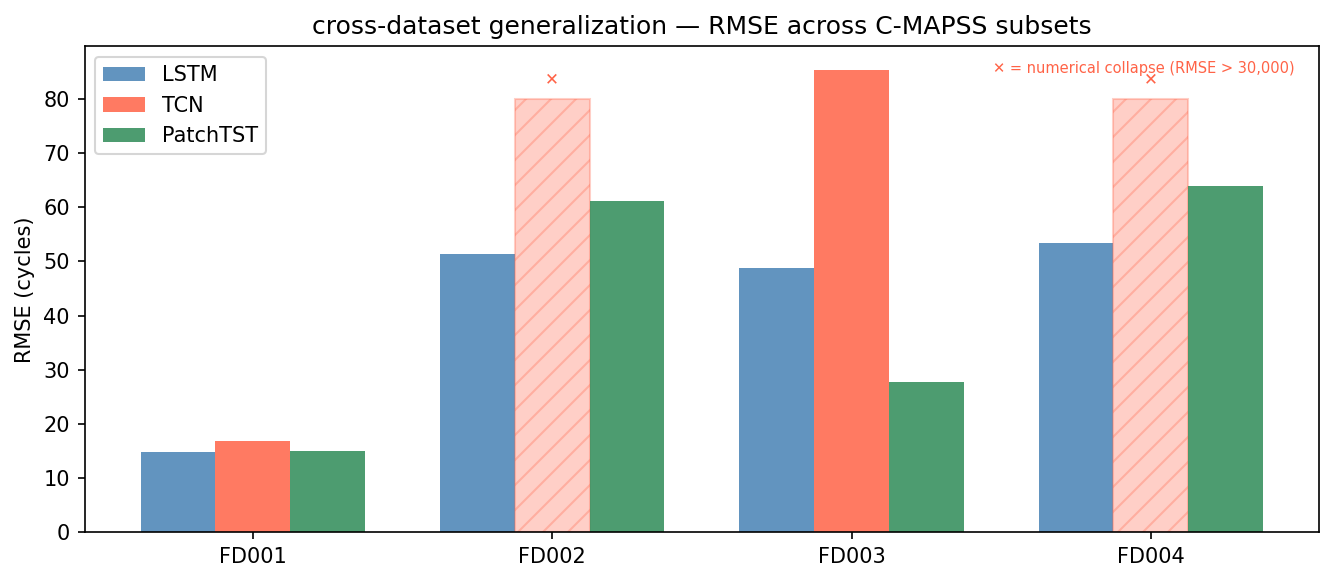
\includegraphics[width=0.88\linewidth]{fig2_cross_dataset.png}
  \caption{Cross-dataset RMSE across all four C-MAPSS subsets. Hatched bars with $\times$ indicate TCN numerical collapse (RMSE $> 30{,}000$). All models trained on FD001 only.}
  \label{fig:cross}
\end{figure}

The LSTM degrades gracefully — RMSE roughly triples on the harder subsets, which is expected when the model encounters operating conditions and fault modes outside its training distribution. PatchTST follows a similar trajectory on FD002 and FD004, but shows a notably strong result on FD003 (27.82 RMSE), where it outperforms the LSTM by 21 cycles. FD003 shares FD001's single operating condition but introduces a second fault mode. This suggests PatchTST's patch-level attention captures signatures of fault-mode-driven degradation that generalize across fault types — likely because patches aggregate local temporal patterns that are fault-mode-relevant, and attention over these patches allows the model to focus on the most informative segments of the degradation history.

The TCN's behavior is the most consequential result. On FD003, which shares FD001's single operating condition, the TCN still functions at 85.35 RMSE — degraded but not catastrophically broken. On FD002 and FD004, which both have six operating conditions, the model collapses completely, producing predictions in the tens of thousands. The pattern is clear: when operating conditions change, the absolute sensor values shift dramatically outside the range seen during FD001 training. The TCN's stacked dilated convolutional filters learned representations tightly coupled to FD001's sensor magnitude ranges. When those ranges shift at test time, activations amplify through the residual path and diverge. The LSTM and PatchTST are more robust because their learned representations encode relative temporal change rather than absolute feature values — the LSTM through sequential hidden state updates, and PatchTST through attention over embedded patch vectors.

This finding has a direct practical implication: deploying a TCN-based RUL model across fleets with different operating conditions requires per-condition normalization or explicit domain adaptation. The LSTM and PatchTST are safer defaults when operating conditions are expected to vary.


\section{Conclusion}

On a fixed operating condition with short 30-cycle windows, the LSTM outperforms both variants — a result that runs against the intuition that newer architectures should improve on simpler ones. The TCN's architectural advantages matter most for longer sequences where vanishing gradients are a real bottleneck, and its regularization is harder to tune when the training set is small. PatchTST closes most of the gap, and its patch-level averaging does help with sensor noise, but not enough to overtake the LSTM on FD001 alone.

The cross-dataset analysis tells the more interesting story. The TCN's collapse under operating condition shift — while LSTM and PatchTST degrade gracefully — is a genuine and practically important finding. PatchTST's strong FD003 transfer hints that local patch representations are more portable across fault modes than recurrent or convolutional alternatives. The overall picture is that architecture choice matters more for robustness than for in-distribution performance: on the in-distribution test set, all three models perform within a couple RMSE cycles of each other, but under distribution shift the differences become dramatic.

Given more time, the most natural next step would be a few-shot fine-tuning experiment: take the FD001-trained models, fine-tune on 10--20 engines from FD002 or FD004, and measure how quickly each architecture adapts. It would also be worth experimenting with longer window sizes, where the TCN's explicit receptive field design would be more genuinely advantageous and the LSTM's vanishing gradient limitation would start to matter.


\section*{Collaboration Statement}

This project was completed individually. Claude (Anthropic) was used as a coding assistant throughout the project — specifically for debugging PyTorch model implementations, structuring the training loop, and suggesting hyperparameter ranges to explore during the TCN tuning process. All model architectures were implemented, run, and verified by the author. All experimental design decisions, result interpretation, and the written report are the author's own work.


\bibliographystyle{unsrtnat}
\bibliography{refs}


\end{document}
